% !TEX root = ./bursty_transcription.tex
\section{Finding the ``right'' model: Bayesian parameter inference}
\label{section_04_bayesian_inference}

In this section we aim to reconcile the thermodynamic and kinetic perspectives
that have been brought to bear on the repressor-operator model. From
Section~\ref{section_02_means}, this reconciliation depends on a key
quantitative question as codified by Eq.~\ref{eq:deltaFR_eq_noneq_equiv}: does
the free energy of repressor binding, as described in the thermodynamic models
and indirectly inferred from gene expression measurements, agree with the
corresponding values of repressor binding and unbinding rates in the kinetic
picture, measured or inferred more directly? In this section we tackle the
statistical inference problem of inferring these repressor rates from
single-cell mRNA counts data. But before we can turn to the full case of simple
repression, we must choose an appropriate model of the constitutive promoter and
infer the parameter values in that model. This is the problem we address first.


\subsection{Parameter inference for constitutive promoters}

From consideration of Fano factors in the previous section, we suspect that
model 5 in Figure~\ref{fig2:constit_cartoons}(A), a one-state bursty model of
constitutive promoters, achieves the right balance of complexity and simplicity,
by allowing both Fano factor $\nu>1$, but also by remedying, by design, the
problems of parameter degeneracy that model 4 in
Figure~\ref{fig2:constit_cartoons}(A) suffered~\cite{Razo-Mejia2020}. We will
test this thoroughly on single-cell mRNA counts for different unregulated
promoters from Jones et.\ al.~\cite{Jones2014}, but first we consider It will be
instructive, however, to first consider the Poisson promoter, model 1 in
Figure~\ref{fig2:constit_cartoons}. As we alluded to earlier, since the Poisson
distribution has a Fano factor $\nu$ strictly equal to 1, and all of the
observed data in Figure~\ref{fig2:constit_cartoons}(B) has Fano factor $\nu>1$,
we might already suspect that this model is incapable of fitting the data. We
will verify that this is in fact the case. Using the same argument we can
immediately rule out models 2 and 3 from Figure~\ref{fig2:constit_cartoons}(A).
These models have Fano factors $\nu\le 1$ meaning they are underdispersed
relative to the Poisson distribution. We will also not explicitly consider model
4 from~\fig{fig2:constit_cartoons}(A) since it was already thoroughly analyzed
in~\cite{Razo-Mejia2020}, and since model 5 can be viewed as a special case of
it.

\mrm{Griffin also feels this paragraph should go. Too many times reminding the 
reader what we are up to. I think he is right.}
Our objective for this section will then be to assess whether or not model 5 is
quantitatively able to reproduce experimental data. In other words, if our claim
is that the level of coarse graining in this model is capable of capturing the
relevant features of the data, then we should be able to find values for the
model parameters that can match theoretical predictions with single-molecule
mRNA count distributions. A natural language for this parameter inference
problem is that of Bayesian probability. We will then build a Bayesian inference
pipeline to fit the model parameters to data. To gain intuition on how this
analysis is done we will begin with the ``wrong'' model 1 in
Figure~\ref{fig2:constit_cartoons}(A). We will use the full dataset of
single-cell mRNA counts from~\cite{Jones2014} used in
Figure~\ref{fig2:constit_cartoons}(B).

\subsubsection{Model 1: Poisson promoter}

Model 1 in Figure~\ref{fig2:constit_cartoons}(A) predicts a  mRNA distribution
whose steady-state solution is given by a Poisson distribution with parameter
$\lambda \equiv r / \gamma$, where $r$ is the mRNA production rate, and $\gamma$
is the mRNA degradation rate~\cite{Sanchez2013}. The goal of our inference
problem is then to find the probability distribution for the parameter value
$\lambda$ given the experimental data. By Bayes' theorem this can be written as
\begin{equation}
p(\lambda \mid D) = {p(D \mid \lambda) p(\lambda) \over p(D)},
\end{equation}
where $D = \{m_1, m_2, \ldots, m_N \}$ are the single-cell mRNA experimental
counts. As is standard we will neglect the denominator $p(D)$ on the right
hand side since it is independent of $\lambda$ and serves only as a
normalization factor.

The steady-state solution for the master equation defines the likelihood term
for a single cell $p(m \mid \lambda)$. What this means is that for a given
choice of parameter $\lambda$, under model 1 of
Figure~\ref{fig2:constit_cartoons}(A), we expect to observe $m$ mRNAs in a
single cell with probability
\begin{equation}
p(m\mid\lambda) = \frac{\lambda^m e^{-\lambda}}{m!}.
\label{eq:poisson_inference010}
\end{equation}
Assuming each cell's mRNA count in our dataset is independent of others, the
likelihood of the full inference problem $p(D\mid\lambda)$ is simply a product
of the single cell likelihoods given by Eq.~\ref{eq:poisson_inference010} above, so
\begin{equation}
p(D\mid\lambda) = \prod_{k=1}^N \frac{\lambda^{m_k}e^{-\lambda}}{m_k!}.
\end{equation}

To proceed we need to specify a prior distribution $p(\lambda)$. In this case we
are extremely data-rich, as the dataset from Jones et.\ al~\cite{Jones2014} has
of order 1000-3000 single-cell measurements for each promoter, so our choice of
prior matters little here, as long as it is sufficiently broad. For details on
the prior selection we refer the reader to Appendix~\ref{sec:bayesian}. For our
purpose here it suffices to specify that we use as prior a Gamma distribution.
This particular choice of prior introduces two new parameters, $\alpha$ and
$\beta$, which parametrize the gamma distribution itself, which we use to encode
the range of $\lambda$ values we view as reasonable. Recall $\lambda$ is the
mean steady-state mRNA count per cell, which \textit{a priori} could plausibly
be anywhere from 0 to a few hundred. $\alpha=1$ and $\beta=1/50$ achieve this,
since the gamma distribution is strictly positive with mean $\alpha/\beta$ and
standard deviation $\sqrt{\alpha}/\beta$.

As detailed in Appendix~\ref{sec:bayesian} this particular choice of prior is
known as the \textit{conjugate} prior for a Poisson likelihood.
Conjugate priors have the convenient properties that a closed form exists for the posterior distribution $p(\lambda \mid D)$ - unusual in Bayesian inference problems - and the closed form posterior takes the same form as the prior. For
our case of a Poisson distribution likelihood with its
Gamma distribution conjugate prior, the posterior distribution is also a Gamma
distribution~\cite{Gelman2013}. Specifically the two parameters $\alpha'$ and
$\beta'$ for this posterior distribution take the form $\alpha' = \alpha +
\bar{m} N$ and $\beta' = \beta + N$, where we defined the sample mean $\bar{m} =
\frac{1}{N}\sum_{k=1}^N m_k$ for notational convenience, and $N$ is the number
of cells in our dataset. Furthermore, given that $N$ is $\mathcal{O}(10^3)$ and
$\langle m\rangle \gtrsim 0.1$ for all promoters measured in~\cite{Jones2014}
our data easily overwhelms the choice of prior, and allows us to approximate the
Gamma distribution with a Gaussian distribution with mean $\bar{m}$ and variance
$\bar{m} / N$ with marginal errors. As an example with real numbers, for the
\textit{lacUV5} promoter, Jones et.\ al~\cite{Jones2014} measured 2648 cells
with an average mRNA count per cell of $\bar{m} \approx 18.7$. For this case our
posterior distribution $P(\lambda \mid D)$ would be a Gaussian distribution with
mean $\mu = 18.7$, and a standard deviation $\sigma \approx 0.08$. This suggests
we have inferred our model's one parameter to a precision of order 1\%.

We remind the reader that we began this section claiming that the Poisson model
was ``wrong'' since it could not reproduce features of the data such as a Fano
factor $> 1$. The fact that we obtain such a narrow posterior distribution for our
parameter $P(\lambda \mid D)$ does not equate to the model being adequate to
describe the data. What this means is that given the data $D$, only values
in a narrow range are remotely plausible for the parameter $\lambda$,
but a narrow posterior distribution does not necessarily
mean the model accurately depicts reality.
As we will see later in Figure~\ref{fig:constit_post_full} after
exploring the bursty promoter model, indeed the correspondence
when contrasting the Poisson model with the experimental data is quite poor.

\subsubsection{Model 5 - Bursty promoter}

Let us now consider the problem of parameter inference for model five
from~\fig{fig1:means_cartoons}(C). As derived in
Appendix~\ref{sec:gen_fcn_appdx}, the steady-state mRNA distribution in this
model is a negative binomial distribution, given by
\begin{equation}
p(m) = \frac{\Gamma(m+k_i)}{\Gamma(m+1)\Gamma(k_i)}
        \left(\frac{1}{1+b}\right)^{k_i}
        \left(\frac{b}{1+b}\right)^m,
\label{eq:neg_bionom}
\end{equation}
where $b$ is the mean burst size and $k_i$ is the burst rate in units of the
mRNA degradation rate $\gamma$. As sketched earlier, to think of the negative
binomial distribution in terms of an intuitive ``story,'' in the precise
meaning of~\cite{Blitzstein2015}, we imagine the arrival of
bursts as a Poisson process with rate $k_i$, where each burst has a
geometrically-distributed size with mean size $b$.

As for the Poisson promoter model, this expression for the steady-state mRNA
distribution is exactly the likelihood we want to use when stating Bayes
theorem. Again denoting the single-cell mRNA count data as $D=\{m_1, m_2,\dots,
m_N\}$, here Bayes' theorem takes the form
\begin{equation}
p(k_i, b \mid D) \propto p(D\mid k_i,b)p(k_i, b).
\end{equation}
We already have our likelihood -- the product of $N$ negative binomials as
Eq.~\ref{eq:neg_bionom} -- so we only need to choose priors on $k_i$ and $b$.
For the datasets from~\cite{Jones2014} that we are analyzing, as for the Poisson
promoter model above we are still data-rich so the prior's influence remains
weak, but not nearly as weak because the dimensionality of our model has
increased from one parameter to two. Details on the arguments behind our prior
distribution selection are left for Appendix~\ref{sec:bayesian}. We state here
that the natural scale to explore these parameters is logarithmic. This is
commonly the case for parameters for which our previous knowledge based on our
domain expertise spans several orders of magnitude. For this we chose log-normal
distributions for both $k_i$ and $b$. Details on the mean and variance of these
distributions can be found in Appendix~\ref{sec:bayesian}.

We carried out Markov-Chain Monte Carlo (MCMC) sampling on the posterior of this
model, starting with the constitutive \textit{lacUV5} dataset
from~\cite{Jones2014}. The resulting MCMC samples are shown in
Figure~\ref{fig:constit_post_full}(A). In contrast to the active/inactive
constitutive model considered in~\cite{Razo-Mejia2020} (nonequilibrium model 4
in Figure~\ref{fig2:constit_cartoons}(A)), this model is well-identified with both
parameters determined to a fractional uncertainty of 5-10\%. The strong
correlation reflects the fact that their product sets the mean of the mRNA
distribution, which is tightly constrained by the data, but there is weak
``sloppiness''~\cite{Transtrum2015} along a set of values with a similar
product.

Having found the model's posterior to be well-identified as with the Poisson
promoter, the next step is to compare both models with experimental data. To do
this for the case of the bursty promoter, for each of the parameter samples
shown in Figure~\ref{fig:constit_post_full}(A) we generated negative
bionomial-distributed mRNA counts. As MCMC samples parameter space
proportionally to the posterior distribution, this set of random samples span
the range of possible values that we would expect given the correspondence
between our theoretical model and the experimental data. A similar procedure can
be applied to the Poisson promoter. To compare so many samples with the actual
observed data, we can use empirical cumulative distribution functions (ECDF) of
the distribution quantiles. This representation is shown in
Figure~\ref{fig:constit_post_full}(B). In this example, the median for each
possible mRNA count for the Poisson distribution is shown as a dark green line,
while the lighter green contains 95\% of the randomly generated samples. This
way of representing the fit of the model to the data gives us a sense of the
range of data we might consider plausible, under the assumption that the model
is true. For this case, as we expected given our premise of the Poisson promoter
being wrong, it is quite obvious that the observed data, plotted in black is not
consistent with the Poisson promoter model. An equivalent plot for the bursty
promoter model is shown in blue. Again the darker tone shows the median, while
the lighter color encompasses 95\% of the randomly generated samples. Unlike the
Poisson promoter model, the experimental ECDF closely tracks the posterior
predictive ECDF, indicating this model is actually able to generate the observed
data and increasing our confidence that this model
is sufficient to parametrize the physical reality of the system.

The commonly used promoter sequence \textit{lacUV5} is our primary
target here, since it forms the core of all the
simple repression constructs of~\cite{Jones2014} that we consider in
Section~\ref{sec:rep_kinetics_inference}. Nevertheless, we thought it wise to
apply our bursty promoter model to the other 17 unregulated promoters available
in the single-cell mRNA count dataset from~\cite{Jones2014} as a test that the
model is capturing the essential phenomenology. If the model fit well to all the
different promoters, this would increase our confidence that it would serve well
as a foundation for inferring repressor kinetics later in
Section~\ref{sec:rep_kinetics_inference}. Conversely, were the model to fail on
more than a couple of the other promoters, it would give us pause.

\begin{figure}%[h!]
\centering
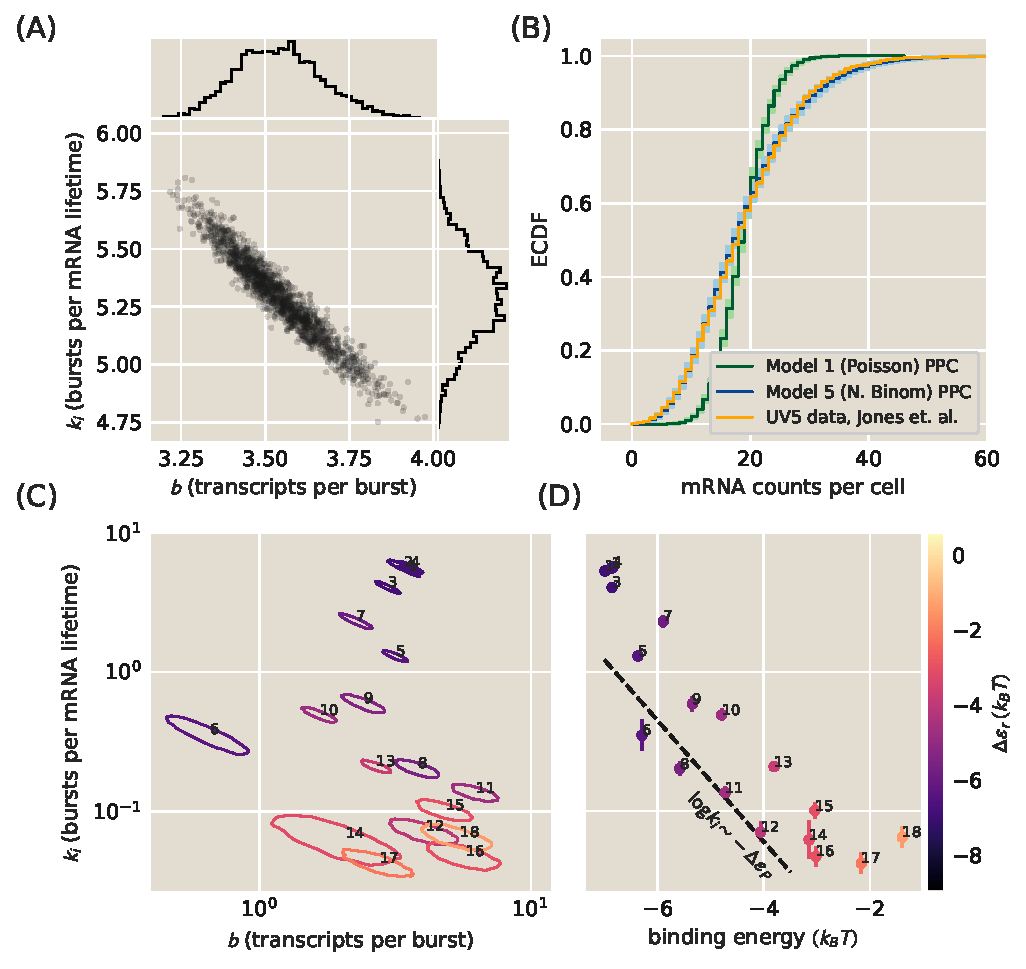
\includegraphics[width=\textwidth]{../../figures/main/fig03.pdf}
\caption{\textbf{Constitutive promoter posterior inference and model
comparison.} (A) The joint posterior density of model 5, the bursty promoter
with negative binomially-distributed steady state, is plotted with MCMC samples.
1D marginal probability densities are plotted as flanking histograms. The model
was fit on \textit{lacUV5} data from~\cite{Jones2014}. (B) The empirical
distribution function (ECDF) of the observed population distribution of mRNA
transcripts under the control of a constitutive \textit{lacUV5} promoter is
shown in black. The median posterior predictive ECDFs for models (1), Poisson,
and (5), negative binomial, are plotted in dark green and dark blue,
respectively. Lighter green and blue regions enclose 95\% of all posterior
predictive samples from their respective models. Model (1) is in obvious
contradiction with the data while model (5) is not. Single-cell mRNA count data
is again from~\cite{Jones2014}. (C) Joint posterior distributions for burst rate
$k_i$ and mean burst size $b$ for 18 unregulated promoters
from~\cite{Jones2014}. Each contour indicates the 95\% highest posterior
probability density region for a particular promoter. Note that the vertical
axis is shared with (D). (D) Plots of the burst rate $k_i$ vs.\ the binding
energy for each promoter as predicted in~\cite{Brewster2012}. The dotted line
shows the predicted slope according to Eq.~\ref{eq:bursty_equil_corresp1},
described in text. Each individual promoter is labeled with a unique number in
both (C) and (D) for cross comparison and for comparison with 
Figure~\ref{fig2:constit_cartoons}(B).}
\label{fig:constit_post_full}
\end{figure}

\fig{fig:constit_post_full}(C) shows the results, plotting the posterior
distribution from individually MCMC sampling all 18 constitutive promoter
datasets from~\cite{Jones2014}. To aid visualization, rather than plotting
samples for each promoter's posterior as in \fig{fig:constit_post_full}(A), for
each posterior we find and plot the curve that surrounds the 95\% highest
probability density region. What this means is that each contour 
encloses approximately 95\% of the samples, and thus 95\% of the probability
mass, of its posterior distribution. Theory-experiment comparisons,
shown in Figure~\ref{figS:ppc_unreg} in Appendix~\ref{sec:bayesian},
display a similar level of agreement between data and predictive samples as for
the bursty model with \textit{lacUV5} in \fig{fig:constit_post_full}(B).

One interesting feature from \fig{fig:constit_post_full}(C) is that burst rate
varies far more widely, over a range of $\sim10^2$, than burst size, confined to
a range of $\lesssim10^1$ (and with the exception of promoter 6, just a span of
3 to 5-fold). This suggests that $k_i$, not $b$, is the key dynamic variable that
promoter sequence tunes.

\subsubsection{Connecting inferred parameters to prior work}
It is interesting to connect these inferences on $k_i$ and $b$ to the work
of~\cite{Brewster2012}, where these same 18 promoters were considered through
the lens of the three-state thermodynamic model (model 2 in
Figure~\ref{fig1:means_cartoons}(B)) and binding energies $\Delta\varepsilon_P$
were predicted from an energy matrix model derived from~\cite{Kinney2010}. As
previously discussed the thermodynamic models of gene regulation can only make
statements about the mean gene expression. This implies that we can draw the
connection between both frameworks by equating the mean mRNA $\left\langle m
\right\rangle$. This results in
\begin{equation}
\langle m \rangle = \frac{k_i b}{\gamma}
        = \frac{r}{\gamma}
        \frac{\frac{P}{N_{NS}}\exp(-\beta\Delta\varepsilon_P)}
                {1+\frac{P}{N_{NS}}\exp(-\beta\Delta\varepsilon_P)}.
\end{equation}
By taking the weak promoter approximation for the equilibrium model ($P/N_{NS} 
\exp(-\beta\Delta\varepsilon_r) \ll 1$) results in~\cite{Brewster2012}
\begin{equation}
\langle m \rangle = \frac{k_i b}{\gamma}
        = \frac{r}{\gamma} \frac{P}{N_{NS}}\exp(-\beta\Delta\varepsilon_P),
\end{equation}
valid for all the binding energies considered here.

Given this result, how are the two coarse-grainings related? A quick estimate
can shed some light. Consider for instance the \textit{lacUV5} promoter, which
we see from Figure~\ref{fig:constit_post_full}(A) has $k_i/\gamma \sim b \sim
\text{few}$, from Figure~\ref{fig:constit_post_full}(B) has $\langle m \rangle
\sim 20$, and from~\cite{Brewster2012} has $\beta\Delta\varepsilon_P \sim -
6.5$. Further we generally assume $P/N_{NS} \sim 10^{-3}$ since
$N_{NS}\approx4.6\times10^6$ and $P\sim10^3$. After some guess-and-check with
these values, one finds the only association that makes dimensional sense and
produces the correct order-of-magnitude for the known parameters is to take
\begin{equation}
\frac{k_i}{\gamma} = \frac{P}{N_{NS}} \exp(-\beta\Delta\varepsilon_P)
\label{eq:bursty_equil_corresp1}
\end{equation}
and
\begin{equation}
b = \frac{r}{\gamma}.
\label{eq:bursty_equil_corresp2}
\end{equation}
Figure~\ref{fig:constit_post_full}(D) shows that this linear scaling between
$\ln k_i$ and $-\beta\Delta\varepsilon_P$ is approximately true for all 18
constitutive promoters considered. The plotted line is simply
Eq.~\ref{eq:bursty_equil_corresp1} and assumes $P\approx 5000$.

While the associations represented by Eq.~\ref{eq:bursty_equil_corresp1} and
Eq.~\ref{eq:bursty_equil_corresp2} appear to be borne out by the data in
Figure~\ref{fig:constit_post_full}, we do not find the association of parameters
they imply to be intuitive. We are also cautious to ascribe too much physical
reality to the parameters. Indeed, part of our point in comparing the various
constitutive promoter models is to demonstrate that these models each provide an
internally self-consistent framework that adequately describes the data, but
attempting to translate between models reveals the dubious physical
interpretation of their parameters.

\mrm{ I would vote to remove this paragraph completely.}
We mention one further comparison, between our inferred parameters and the work
of Chong et.\ al.~\cite{Chong2014}, which is interesting and puzzling.
Experiments in~\cite{Chong2014} convincingly argue that supercoiling accumulated
from the production of mRNA transcripts is key in setting the burstiness of mRNA
production. In their model, this supercoiling occurs on the scale of
$\sim100$~kb domains of DNA. This suggests that all genes on a given domain
should burst in synchrony, and that the difference between highly and lowly
expressed genes is the \textit{size} of transcriptional bursts, not the
\textit{time between} bursts. But here, all burst sizes we infer in
Figure~\ref{fig:constit_post_full}(C) are comparable and burst rates vary
wildly. It is not immediately clear how to square this circle. Furthermore,
Figure~7E in~\cite{Chong2014} reports values of the quantity they label
$\beta/\alpha$ and we label $k^+/k^-$ in model 4 from
Figure~\ref{fig2:constit_cartoons}. In contrast to the findings
of~\cite{Razo-Mejia2020}, Chong et.\ al.\ do not find $k^+/k^-\ll1$ for most of
the genes they consider. This begs the question: is the \textit{galK}
chromosomal locus used for the reporter constructs in~\cite{Razo-Mejia2020}
and~\cite{Jones2014} merely an outlier, or is there a deeper puzzle here waiting
to be resolved? Without more apples-to-apples data we can only speculate, and we
leave it as an intriguing open question for the field.

Despite such puzzles, our goal here is not to unravel the mysterious origins of
burstiness in transcription. Our remaining task in this work is a determination
of the physical reality of thermodynamic binding energies in
Figure~\ref{fig1:means_cartoons}, as codified by the thermodynamic-kinetic
equivalence of Eq.~\ref{eq:deltaFR_eq_noneq_equiv}. For our phenomenological
needs here model 5 in Figure~\ref{fig2:constit_cartoons}(A) is more than
adequate: the posterior distributions in Figure~\ref{fig:constit_post_full}(C)
are cleanly identifiable and the predictive checks in
Figure~\ref{figS:ppc_unreg} indicate no discrepancies between the model and the
mRNA single-molecule count data of~\cite{Jones2014}. Of the models we have
considered it is unique in satisfying both these requirements. So we will
happily use it as a foundation to build upon in the next section when we add
regulation.

\subsection{Transcription factor kinetics can be inferred from single-cell mRNA
distribution measurements}\label{sec:rep_kinetics_inference}
\subsubsection{Building the model and performing parameter inference}

Now that we have a satisfactory model in hand for constitutive promoters, we
would like to return to the main thread: can we reconcile the thermodynamic and
kinetic models by putting to the test Eq.~\ref{eq:deltaFR_eq_noneq_equiv}, the
correspondence between indirectly inferred thermodynamic binding energies and
kinetic rates? To make this comparison, is it possible to infer repressor
binding and unbinding rates from mRNA distributions over a population of cells
as measured by single-molecule Fluorescence \textit{in situ} Hybridization
in~\cite{Jones2014}? If so, how do these inferred rates compare to direct
single-molecule measurements such as from~\cite{Hammar2014} and to binding
energies such as from~\cite{Garcia2011a} and~\cite{Razo-Mejia2018}, which were
inferred under the assumptions of the thermodynamic models in
Figure~\ref{fig1:means_cartoons}(B)? And can this comparison shed light on the
unreasonable effectiveness of the equilibrium models, for instance, in their
application in~\cite{Chure2019, Chure2019a}?

\begin{figure}%[h!]
\centering
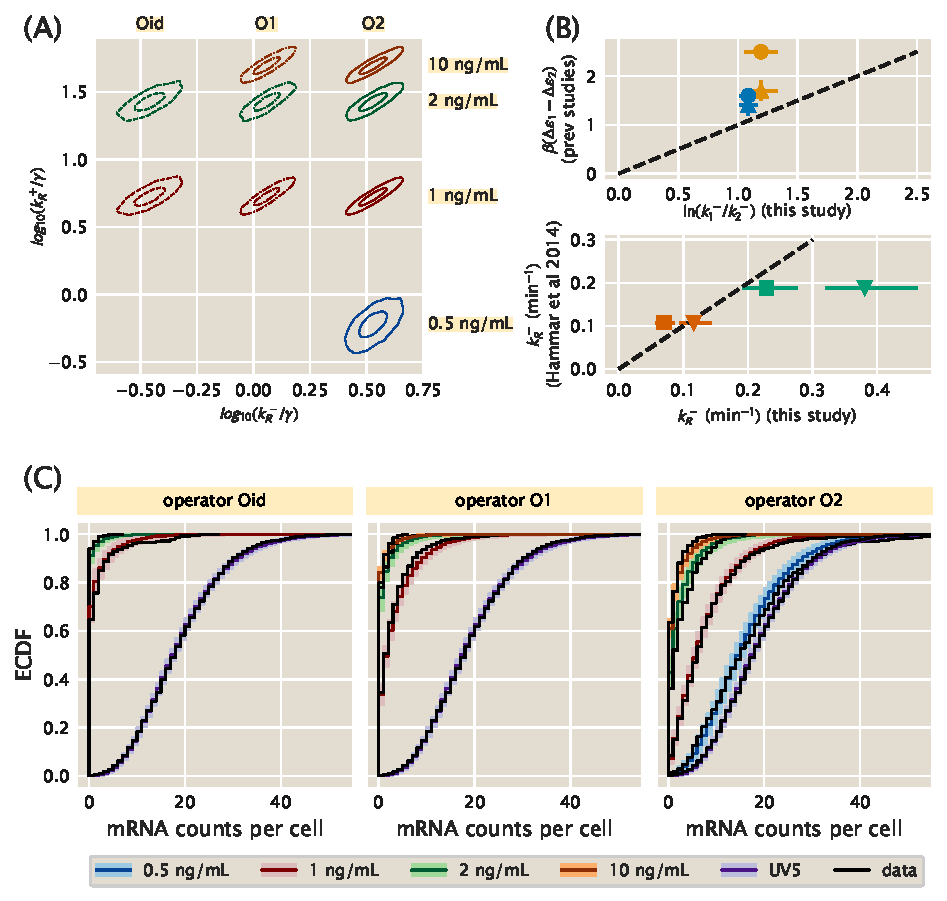
\includegraphics[width=\textwidth]{../../figures/main/fig04.pdf}
\caption{\textbf{Simple repression parameter inference and comparison.}
(A) Contours which enclose 50\% and 95\% of the posterior probability mass are
shown for each of several 2D slices of the 9D posterior distribution. The model
assumes one unbinding rate for each operator (Oid, O1, O2) and one binding rate
for each aTc induction concentration (corresponding to an unknown mean repressor
copy number).
(B, upper) Ratios of our inferred unbinding rates are
compared with operator binding energy differences measured by Garcia and
Phillips~\cite{Garcia2011a} (triangles) and Razo-Mejia et.\
al.~\cite{Razo-Mejia2018} (circles). Blue glyphs compare O2-O1, while orange
compare O1-Oid. Points with perfect agreement would lie on the dotted line.
(B, lower) Unbinding rates for O1 (cyan) and Oid (red)
inferred in this work are compared with single-molecule measurements
from Hammar et.\ al.~\cite{Hammar2014}. We plot the comparison assuming illustrative mRNA
lifetimes of $\gamma^{-1}=3$~min (triangles) or $\gamma^{-1}=5$~min
(squares). Dotted line is as in upper panel.
(C) Theory-experiment comparison are shown for each of the datasets
used in the inference of the model in (A). Observed single-molecule mRNA counts
data from~\cite{Jones2014} are plotted as black lines. The median of the randomly
generated samples for each condition is plotted as a dark colored line. Lighter
colored bands enclose 95\% of all samples for a given operator/repressor copy
number pair.
%Samples are sorted by operator and plotted separately for visual clarity.
The unregulated promoter, \textit{lacUV5}, is shown with each as a reference.}
\label{fig4:repressed_post_full}
\end{figure}

As we found in Section~\ref{sec:beyond_means}, for our purposes the ``right''
model of a constitutive promoter is the bursty picture, model five in
Figure~\ref{fig2:constit_cartoons}(A). Therefore our starting point here is the
analogous model with repressor added, model 5 in
Figure~\ref{fig1:means_cartoons}(C). For a given repressor binding site and copy
number, this model has four rate parameters to be inferred: the repressor
binding and unbinding rates $k_R^+$, and $k_R^-$, the initiation rate of bursts,
$k_i$, and the mean burst size $b$ (we nondimensionalize all of these by the
mRNA degradation rate $\gamma$).

Before showing the mathematical formulation of our statistical inference model,
we would like to sketch the intuitive structure. The dataset
from~\cite{Jones2014} we consider consists of single-cell mRNA counts data of
nine different conditions, spanning several combinations of three unique
repressor binding sites (the so-called $Oid$, $O1$, and $O2$ operators) and four
unique repressor copy numbers. We assume that the values of $k_i$ and $b$ are
known, since we have already cleanly inferred them from constitutive promoter
data, and further we assume that these values are the same across datasets with
different repressor binding sites and copy numbers. In other words, we assume
that the regulation of the transcription factor does not affect the mean burst
size nor the burst initiation rate. The regulation occurs as the promoter is
taken away from the transcriptionally active state when the promoter is bound by
repressor. We assume that there is one unbinding rate parameter for each
repressor binding site, and likewise one binding rate for each unique repressor
copy number. This makes our model seven dimensional, or nine if one counts $k_i$
and $b$ as well. Note that we use only a subset of the datasets from Jones et.\
al.~\cite{Jones2014}, as discussed more in Appendix~\ref{sec:bayesian}.

Formally now, denote the set of seven repressor rates to be inferred as
\begin{equation}
\vect{k} =\{k_{Oid}^-, k_{O1}^-, k_{O2}^-,
k_{0.5}^+, k_{1}^+, k_{2}^+, k_{10}^+\},
\end{equation}
where subscripts for dissociation rates $k^-$  indicate the different repressor
binding sites, and subscripts for association rates $k^+$ indicate the
concentration of the small-molecule that controlled the expression of the LacI
repressor (see Appendix~\ref{sec:bayesian}). This is because for this particular
dataset the repressor copy numbers were not measured directly, but it is safe to
assume that a given concentration of the inducer resulted in a specific mean
repressor copy number~\cite{Chure2019a}. Also note that the authors
of~\cite{Jones2014} report estimates of LacI copy number per cell rather than
direct measurements. However, these estimates were made assuming the validity of
the thermodynamic models in Figure~\ref{fig1:means_cartoons}, and since testing
these models is our present goal, it would be circular logic if we were to make
the same assumption. Therefore we will make no assumptions about the LacI copy
number for a given inducer concentration.

Having stated the problem, Bayes' theorem reads
\begin{equation}
p(\vect{k}, k_i, b \mid D)
\propto
p(D \mid\vect{k}, k_i, b) p(\vect{k}, k_i, b),
\end{equation}
where $D$ is again the set of all $N$ observed single-cell mRNA counts
across the various conditions. We assume that individual single-cell
measurements are independent so that the likelihood factorizes as
\begin{equation}
p(D \mid\vect{k}, k_i, b)
= \prod_{j=1}^N p(m\mid \vect{k}, k_i, b)
= \prod_{j=1}^N p(m\mid k_j^+, k_j^-, k_i, b)
\end{equation}
where $k_j^\pm$ represent the appropriate binding and unbinding
rates out of $\vect{k}$ for the $j$-th measured cell. The probability
$p(m\mid k_j^+, k_j^-, k_i, b)$ appearing in the last expression
is exactly Eq.~\ref{eq:p_m_bursty+rep_appdx}, the steady-state
distribution for our bursty model with repression derived in
Section~\ref{sec:gen_fcn_appdx}, which for completeness we reproduce here as
\begin{equation}
\begin{split}
p(m \mid k_R^+, k_R^-, k_i, b) = & ~\frac{
        \Gamma(\alpha + m)\Gamma(\beta + m)\Gamma(k_R^+ + k_R^-)
        }
        {
        \Gamma(\alpha)\Gamma(\beta)\Gamma(k_R^+ + k_R^- + m)
        }
\frac{b^m}{m!}
\\
&\times {_2F_1}(\alpha+m, \beta+m, k_R^++k_R^-+m; -b).
\end{split}
\label{eq:p_m_bursty+rep}
\end{equation}
where $_2F_1$ is the confluent hypergeometric function of the second kind and
$\alpha$ and $\beta$, defined for notational convenience, are
\begin{align}
\begin{split}
\alpha &= \frac{1}{2}
\left(k_i+k_R^-+k_R^+ + \sqrt{(k_i+k_R^-+k_R^+)^2 - 4k_i k_R^-}\right)
\\
\beta &= \frac{1}{2}
\left(k_i+k_R^-+k_R^+ - \sqrt{(k_i+k_R^-+k_R^+)^2 - 4k_i k_R^-}\right).
\end{split}
\end{align}

This likelihood is rather inscrutable. We did not find any of the known
analytical approximations for ${_2F_1}$ terribly useful in gaining intuition, so
we instead resorted to numerics. One insight we found
was that for very strong or very weak repression, the distribution in
Eq.~\ref{eq:p_m_bursty+rep} is well approximated by a negative binomial with
burst size $b$ and burst rate $k_i$ equal to their constitutive \textit{lacUV5}
values, except with $k_i$ multiplied by the fold-change
$\left(1+k_R^+/k_R^-\right)^{-1}$. In other words, once again only the ratio
$k_R^+/k_R^-$ was detectable. But for intermediate repression, the distribution
was visibly broadened with Fano factor greater than $1+b$, the value for the
corresponding constitutive case. This indicates that the repressor rates had
left an imprint on the distribution, and perhaps intuitively, this intermediate
regime occurs for values of $k_R^\pm$ comparable to the burst rate $k_i$. Put
another way, if the repressor rates are much faster or much slower than $k_i$,
then there is a timescale separation and effectively only one timescale remains,
$k_i\left(1+k_R^+/k_R^-\right)^{-1}$. Only when all three rates in the problem
are comparable does the mRNA distribution retain detectable information about
them.

Next we specify priors. As for the constitutive model, weakly informative
log-normal priors are a natural choice for all our rates. We found that if the
priors were too weak, our MCMC sampler would often become stuck in regions of
parameter space with very low probability density, unable to move. We struck a
balance in choosing our prior widths between helping the sampler run while
simultaneously verifying that the marginal posteriors for each parameter were
not artificially constrained or distorted by the presence of the prior.
% The only
% exception to this is the highly informative priors we placed on $k_i$ and $b$,
% since we have strong knowledge of them from our inference of constitutive
% promoters above.
All details for our prior distributions are listed in 
Appendix~\ref{sec:bayesian}.

We ran MCMC sampling on the full nine dimensional posterior specified by this
model. To attempt to visualize this object, in
Figure~\ref{fig4:repressed_post_full}(A) we plot several two-dimensional slices
as contour plots, analogous to Figure~\ref{fig:constit_post_full}(C). Each of
these nine slices corresponds to the $(k_R^+, k_R^-)$ pair of rates for one of
the conditions from the dataset used to fit the model and gives a
sense of the uncertainty and correlations in the posterior.
We note that the 95\% uncertainties of all the rates span about $\sim0.3$
log units, or about a factor of two, with the exception of $k_{0.5}^+$, the
association rate for the lowest repressor copy number which is somewhat larger.

\subsubsection{Comparison with prior measurements of repressor binding energies}
Our primary goal in this work is to reconcile the kinetic and thermodynamic
pictures of simple repression. Towards this end we would like to compare the
repressor kinetic rates we have inferred with the repressor binding energies
inferred through multiple methods in~\cite{Garcia2011a}
and~\cite{Razo-Mejia2018}. If the agreement is close, then it suggests that the
thermodynamic models are not wrong and the repressor binding energies they
contain correspond to physically real free energies, not mere fit parameters.

Figure~\ref{fig4:repressed_post_full}(B) shows both comparisons, with the top
panel comparing to thermodynamic binding energies and the bottom panel comparing
to single-molecule measurements. First consider the top panel and its comparison
between repressor kinetic rates and binding energies. As described in
section~\ref{section_02_means}, if the equilibrium binding energies
from~\cite{Garcia2011a} and~\cite{Razo-Mejia2018} indeed are the physically real
binding energies we believe them to be, then they should be related to the
repressor kinetic rates via Eq.~\ref{eq:deltaFR_eq_noneq_equiv}, which we
restate here,
\begin{equation}
\Delta F_R = \beta\Delta\varepsilon_R - \log(R/N_{NS})
        = - \log(k_R^+/k_R^-).
\label{eq:deltaFR_eq_noneq_equiv_repeat}
\end{equation}
Assuming mass action kinetics implies that $k_R^+$ is proportional to repressor
copy number $R$, or more precisely, it can be thought of as repressor copy
number times some intrinsic per molecule association rate. But since $R$ is not
directly known for our data from~\cite{Jones2014}, we cannot use this equation
directly. Instead we can consider two different repressor binding sites and
compute the \textit{difference} in binding energy between them, since this
difference depends only on the unbinding rates and not on the binding rates.
This can be seen by evaluating Eq.~\ref{eq:deltaFR_eq_noneq_equiv_repeat} for
two different repressor binding sites, labeled (1) and (2), but with the same
repressor copy number $R$, and taking the difference to find
\begin{equation}
\Delta F_R^{(1)} - \Delta F_R^{(2)}
= \beta\Delta\varepsilon_1 - \beta\Delta\varepsilon_2
= - \log(k_R^+/k_1^-) + \log(k_R^+/k_2^-),
\end{equation}
or simply
\begin{equation}
\beta\Delta\varepsilon_1 - \beta\Delta\varepsilon_2
= \log(k_2^-/k_1^-).
\end{equation}
The left and right hand sides of this equation are exactly the horizontal and
vertical axes of the top panel of Figure~\ref{fig4:repressed_post_full}. Since
we inferred rates for three repressor binding sites (O1, O2, and Oid), there are
only two independent differences that can be constructed, and we arbitrarily
chose to plot O2-O1 and O1-Oid in Figure~\ref{fig4:repressed_post_full}(B).
Numerically, we compute values of $k_{O1}^- / k_{Oid}^-$ and $k_{O2}^- /
k_{O1}^-$ directly from our full posterior samples, which conveniently provides
uncertainties as well, as detailed in Appendix~\ref{sec:bayesian}.
% \mmnote{Explain in appendix how marginalization with sampling makes this
% ``trivial'' to compute from samples of the joint posterior, b/c sampling makes
% marginalization trivial.}
We then compare these log ratios of rates to the
binding energy differences $\Delta\varepsilon_{O1} - \Delta\varepsilon_{Oid}$
and from $\Delta\varepsilon_{O2} - \Delta\varepsilon_{O1}$ as computed from the
values from both~\cite{Garcia2011a} and~\cite{Razo-Mejia2018}. Three of the four
values are within $\sim0.5~k_BT$ of the diagonal representing perfect agreement,
which is comparable to the $\sim\text{few}\times0.1~k_BT$ variability between
the independent determinations of the same quantities between~\cite{Garcia2011a}
and~\cite{Razo-Mejia2018}. The only outlier involves Oid measurements
from~\cite{Razo-Mejia2018}, and as the authors of~\cite{Razo-Mejia2018} note,
this is a difficult measurement of low fluorescence signal against high
background since Oid represses so strongly. We are therefore inclined to regard
the failure of this point to fall near the diagonal as a testament to the
difficulty of the measurement and not as a failure of our theory.

On the whole then, we regard this as striking confirmation of the validity of
the equilibrium models. Their lynchpin parameter is a phenomenological free
energy of repressor binding that has previously only been inferred indirectly.
Our result shows that the microscopic interpretation of this free energy, as the
log of a ratio of transition rates, does indeed hold true to within the inherent
uncertainties that remain in the entire theory-experiment dialogue.
%\mmnote{Does this deserve qualifiers, like ``to a good approximation,'' or ``as a first order model'' or something? I like the simple finality without, but I worry it's too brazen or subtlely misleading.}

\subsubsection{Comparison with prior measurements of repressor kinetics}
In the previous section we established the equivalence between the equilibrium
models' binding energies and the repressor kinetics we infer from mRNA
population distributions. But one might worry that the repressor rates we infer
from mRNA distributions are \textit{themselves} merely fitting parameters and
that they do not actually correspond to the binding and unbinding rates of the
repressor in vivo. To verify that this is not the case, we next compare our
kinetic rates with a different measurement of the same rates using a radically
different method: single molecule measurements as performed in Hammar et.\
al.~\cite{Hammar2014}. This is plotted in the lower panel of
Figure~\ref{fig4:repressed_post_full}(B).

Since we do not have access to repressor copy number for either the
single-cell mRNA data from~\cite{Jones2014} or the single-molecule data
from~\cite{Hammar2014}, we cannot make an apples-to-apples comparison of
association rates $k_R^+$. Further, while Hammar et.\ al.\ directly measure the
dissociation rates $k_R^-$, our inference procedure returns $k_R^-/\gamma$,
i.e., the repressor dissociation rate nondimensionalized by the mRNA degradation
rate $\gamma$. So to make the comparison, we must make an assumption for the
value of $\gamma$ since it was not directly measured. For most mRNAs in
\textit{E.\ coli}, quoted values for the typical mRNA lifetime $\gamma^{-1}$
range between about 2.5~min~\cite{Chen2015} to 8~min. We chose $\gamma^{-1} =
3$~min and $\gamma^{-1} = 5$~min as representative values and plot a comparison
of $k_{O1}^-$ and $k_{Oid}^-$ from our inference with corresponding values
reported in~\cite{Hammar2014} for both these choices of $\gamma$.

The degree of quantitative agreement in the lower panel of
Figure~\ref{fig4:repressed_post_full}(B) clearly depends on the precise choice
of $\gamma$. Nevertheless we find this comparison very satisfying, when two
wildly different approaches to a measurement of the same quantity yield broadly
compatible results. We emphasize the agreement between our rates and the rates
reported in~\cite{Hammar2014} for any reasonable $\gamma$: values differ by at
most a factor of 2 and possibly agree to within our uncertainties of 10-20\%.
From this we feel confident asserting that the parameters we have inferred from
Jones et.\ al.'s single-cell mRNA counts data do in fact correspond to repressor
binding and unbinding rates, and therefore our conclusions on the agreement of
these rates with binding energies from~\cite{Garcia2011a}
and~\cite{Razo-Mejia2018} are valid.

\subsubsection{Model checking}
In Figure~\ref{fig:constit_post_full}(B) we saw that the simple Poisson model of
a constitutive promoter, despite having a well behaved posterior, was clearly
insufficient to describe the data. It behooves us to carry out a similar check
for our model of simple repression, codified by Eq.~\ref{eq:p_m_bursty+rep} for
the steady-state mRNA copy number distribution. As derived in
Sections~\ref{section_02_means} and~\ref{sec:beyond_means}, we have compelling
theoretical reasons to believe it is a good model, but if it nevertheless turned
out to be badly contradicted by the data we should like to know.

The details are deferred to Appendix~\ref{sec:bayesian}, and here we only
attempt to summarize the intuitive ideas, as detailed at greater length by
Jaynes~\cite{Jaynes2003} as well as Gelman and
coauthors~\cite{Gelman2013,Gelman2013a}. From our samples of the posterior
distribution, plotted in Figure~\ref{fig4:repressed_post_full}(A), we generate
many replicate data using a random number generator. In
Figure~\ref{fig4:repressed_post_full}(C), we plot empirical cumulative
distribution functions of the middle 95\% quantiles of these replicate data with
the actual experimental data from Jones et.\ al.~\cite{Jones2014} overlaid,
covering all ten experimental conditions spanning repressor binding sites and
copy numbers (as well as the constitutive baseline UV5).

The purpose of Figure~\ref{fig4:repressed_post_full}(C) is simply a graphical,
qualitative assessment of the model: do the experimental data systematically
disagree with the simulated data, which would suggest that our model is missing
important features? A further question is not just whether there is a detectable
difference between simulated and experimental data, but whether this difference
is likely to materially affect the conclusions we draw from the posterior in
Figure~\ref{fig4:repressed_post_full}(A). More rigorous and quantitative
statistical tests are possible~\cite{Gelman2013}, but their quantitativeness
does not necessarily make them more useful. As stated in~\cite{Gelman2013a}, we
often find this graphical comparison more enlightening because it better engages
our intuition for the model, not merely telling \textit{if} the model is wrong
but suggesting \textit{how} the model may be incomplete.

Our broad brush takeaway from Figure~\ref{fig4:repressed_post_full}(C) is
overall of good agreement. There some oddities, in particular the long tails in
the data for Oid, 1~ng/mL, and O2, 0.5~ng/mL. The latter is especially odd since
it extends beyond the tail of the unregulated UV5 distribution. This is a
relatively small number of cells, however, so whether this is a peculiarity of
the experimental data, a statistical fluke of small numbers, or a real
biological effect is unclear. It is conceivable that there is some very slow
timescale switching dynamics that could cause this bimodality, although it is
unclear why it would only appear for specific repressor copy numbers. There is
also a small offset between experiment and simulation for O2 at the higher
repressor copy numbers, especially at 2 and 10~ng/mL. From the estimate of
repressor copy numbers from~\cite{Jones2014}, it is possible that the repressor
copy numbers here are becoming large enough to partially invalidate our
assumption of a separation of timescales between burst duration and repressor
association rate. Another possibility is that the very large number of zero mRNA
counts for Oid, 2~ng/mL is skewing its partner datasets through the shared
association rate. None of these fairly minor potential caveats cause us to
seriously doubt the overall correctness of our model, which further validates
its use to compare the equilibrium models' binding energies to the
nonequilibrium models' repressor kinetics, as we originally set out to do.